\documentclass[conference]{IEEEtran}
\IEEEoverridecommandlockouts
% The preceding line is only needed to identify funding in the first footnote. If that is unneeded, please comment it out.
\usepackage{cite}
\usepackage{amsmath,amssymb,amsfonts}
%\usepackage{algorithmic}
\usepackage{graphicx}
\usepackage{textcomp}
\usepackage{xcolor}
\def\BibTeX{{\rm B\kern-.05em{\sc i\kern-.025em b}\kern-.08em
    T\kern-.1667em\lower.7ex\hbox{E}\kern-.125emX}}
    
\usepackage{graphicx}
% Used for displaying a sample figure. If possible, figure files should
% be included in EPS format.
%
% If you use the hyperref package, please uncomment the following line
% to display URLs in blue roman font according to Springer's eBook style:
% \renewcommand\UrlFont{\color{blue}\rmfamily}
\usepackage{algorithm}
\usepackage[noend]{algpseudocode}
\usepackage{xcolor}
\usepackage{listings}
\usepackage[most]{tcolorbox}
\usepackage{tabularx}
\usepackage{multirow}
\usepackage{url}

\expandafter\def\expandafter\UrlBreaks\expandafter{\UrlBreaks%  save the current one
  \do\a\do\b\do\c\do\d\do\e\do\f\do\g\do\h\do\i\do\j%
  \do\k\do\l\do\m\do\n\do\o\do\p\do\q\do\r\do\s\do\t%
  \do\u\do\v\do\w\do\x\do\y\do\z\do\A\do\B\do\C\do\D%
  \do\E\do\F\do\G\do\H\do\I\do\J\do\K\do\L\do\M\do\N%
  \do\O\do\P\do\Q\do\R\do\S\do\T\do\U\do\V\do\W\do\X%
  \do\Y\do\Z}

\definecolor{commentgreen}{rgb}{0.3,0.5,0.5}
\definecolor{keyred}{rgb}{0.63,0.129,0.258}
\definecolor{codegray}{rgb}{0.1,0.1,0.1}
\definecolor{codepurple}{rgb}{0.58,0.4,0.82}
\definecolor{backcolour}{rgb}{0.95,0.95,0.92}
%\definecolor{maroon}{cmyk}{0,0.87,0.68,0.32}
\definecolor{maroon}{rgb}{0.87,0.68,0.32}

\usepackage{soul}
\newcommand{\authnote}[2]{{\bf \textcolor{blue}{#1}: \em \textcolor{red}{#2}}}
\newcommand{\baigd}[1]{\authnote{baigd}{#1}}
\newcommand{\add}[1]{\textcolor{blue}{#1}}
\newcommand{\remove}[1]{\textcolor{red}{\st{#1}}}
\newcommand{\replace}[2]{\textcolor{red}{\st{#1}} \textcolor{blue}{#2}}
\newcommand{\highlight}[1]{\textcolor{orange}{#1}}

\lstdefinelanguage{JavaScript}{
  keywords={typeof, new, true, false, catch, return, null, catch, switch, var, if, in, while, do, else, case, break, require, uint, assert, address},
  keywordstyle=\color{blue}\bfseries,
  ndkeywords={class, export, boolean, throw, implements, import, this, function},
  ndkeywordstyle=\color{darkgray}\bfseries,
  identifierstyle=\color{black},
  sensitive=false,
  comment=[l]{//},
  morecomment=[s]{/*}{*/},
  commentstyle=\color{purple}\ttfamily,
  stringstyle=\color{red}\ttfamily,
  morestring=[b]',
  morestring=[b]"
}

\lstdefinestyle{mystyle}{
%  	backgroundcolor=\color{backcolour},
	language=JavaScript,   
    commentstyle=\itshape\color{commentgreen},
    keywordstyle=\bfseries\color{keyred},
    numberstyle=\small,
    stringstyle=\color{codepurple},
	basicstyle=\small,
    breakatwhitespace=false,         
    breaklines=true,                 
    captionpos=b,                    
    keepspaces=true,                 
    numbers=left,                    
    numbersep=2pt,                  
    showspaces=false,                
    showstringspaces=false,
    showtabs=false,                  
    tabsize=2,
    frame={bottomline}
}
\lstset{style=mystyle}

\newcommand{\littlesmall}[1]{\scalebox{0.9}{#1}}
\newcommand{\smalltt}[1]{{\littlesmall{\texttt{#1}}}}
\newcommand{\code}[1]{{\fontfamily{cmtt}\fontseries{m}\fontshape{n}\selectfont\small{#1}}}

\newcommand{\oursystemtext}{XXX}
\newcommand{\oursystem}{\code{{\oursystemtext}}}
\newcommand*{\prompt}[1]{\textsf{\textbf{#1}}}
\newcommand{\tab}{\hspace*{1em}}

\newcommand{\he}[1]{{\color{blue} Ningyu: #1}}
\newcommand{\ji}[1]{{\color{purple} Ru: #1}}
\newcommand{\lei}[1]{{\color{red} Lei: #1}}
\newcommand{\haoyu}[1]{{\color{red} HW: #1}}
\usepackage{xspace}
\usepackage{booktabs}

    
  
\begin{document}

\title{Characterizing Crowdsourcing Based Bitcoin Illicit Address}




\maketitle

\begin{abstract}

\end{abstract}

%%\begin{IEEEkeywords}
%%keywords
%%\end{IEEEkeywords}

\section{Introduction}
\label{sec:intro}

% bitcoin history, bitcoin is different from other sc-based. cryptocurrencies.
Almost 12 years since bitcoin\cite{nakamoto2019bitcoin} was first mined, blockchain, which is an idea that became popular along with, has been growing super fast. There are  10,862 different cryptocurrencies for trade by 5th July, 2021, with a total market cap of \$1,364,980,204,657 \cite{coinmarketcap}. While there are a lot of other cryptocurrencies, bitcoin is still one of the most popular one, which dominated more than 60\% of the market \cite{coinmarketcap}.
%Bitcoin anonymity -> anonymity lead to scam
Anonymous is one of the most important features in Bitcoin. It ensures that it's hard to link bitcoin addresses with real-world entities, so that the information security of users is guaranteed. But at the same time, anonymity makes it easy to commit a crime without easily getting caught, therefore, bitcoin becomes a suitable tool for abuser to collect money from scams. When two users trade using bitcoin, the addresses of bitcoin is the only information provided, so it is hard to track who is behind the scams. Up to today, there are already many kinds of scams using bitcoin as a way to collect scam money. One of the most popular type is sextortion. Although sextortion is a new scheme, it has taken a large percentage in bitcoin scams. The abuser will normally send an email which claims they are in control of the victim's computer or contact list, and will make some compromising images public unless some amount of bitcoin is paid on time\cite{paquet2019spams}. Apart from sextortion, other new schemes continue to come into our sight. During the current pandemic time, various COVID-19 themed scams have emerged. Some abuser created new types of scams based on COVID-19 topics. For example, during July in 2020, some of the celebrities' twitter account have been hacked and posted information claiming to be giving back to community because of COVID-19, but one has to transfer a given amount of bitcoin to the address provided first, the hacker earned more than 10 bitcoin just from Barack Obama's twitter account\cite{barackobamascam}. 
% The damage of BTC scam. The urgent to analyse it.
The above examples show that the scams in Bitcoin is very harmful in the Bitcoin community, it can cause huge damage in personal property. It is urgent to comprehensively understand scams in bitcoin, and at the same time prevent more people from getting scammed. Firstly, a dataset should be constructed, then the features of the scam should be analysed to shed light on the scam schemes. Further, based on the feature extracted, there can be a method to detect more scam addresses. Few works published have focus on this topic, there still lacks a comprehensive understanding of Bitcoin scams.


\textbf{This Paper.}
% Describe the process of the experiment
\begin{itemize}
    \item \textbf{Dataset} 
    
    In this paper, we firstly collect scam addresses from bitcoinabuse.com\cite{bitcoinabuse}, there are 174,404 reports in out dataset. After filtering the repeated ones, we got 50,522 unique addresses.
    \item \textbf{Distribution} 
     The dataset also contains some information describing the features of the abuser. We analysed these information: the email addresses used by the abuser, and the url from which the victims get in touch with the scam, to find out how the scam information is distributed to victims. 
     
     
     \item \textbf{Dataset Expension}
     For the further analysis, we firstly filtered the unique addresses by if they have transactions, then we clean the dataset to remove the falsely reported addresses, with the help of PeckShield. Now our dataset contains 6,004 scam addresses. To prepare for the later detection step, we also collected 6,014 licit addresses. There are a total of 12,018 labelled addresses in our dataset. As we want to explorer the money-flow features of these addresses, we also collected 4,754,462 unlabelled addresses, these unlabelled addresses have direct transaction connection with the labelled addresses. 
     \item \textbf{Clustering}
      In this step, we firstly implemented multi-input clustering, the result shows, then we implemented the previous collected information to further cluster the addresses. We used the email information in the clustering. If multiple BTC addresses use the same email address to distribute the scams, we consider these addresses to be in the same cluster. In the end, we find out the top 10 clusters received a total of 1,620,599.08 bitcoins, the biggest cluster contains 136,309 addresses.
     
     \item \textbf{Detection}
     In this section, we firstly implement traditional machine learning classification algorithm, then we explorer building a graph neural network which can take the graph structure of the dataset into consideration. The graph method is divided into supervised classification and semi-supervised classification. The result shows that our dataset can be used to perform classification with accuracy higher than 93\%, except for the semi-supervised situation.
\end{itemize}






\section{Background}
\label{sec:background}
\subsection{Bitcoin}

\textbf{Transaction} Transaction descibes the money flow from input addresses to output addresses. There are two popular ways to keep record in blockchain network. Account/Balance model is used in Ethereum, it is also the model we often encounter in our daily life, Bank, Paypal, etc, all implements such a model. Bitcoin, however, employs another model called UTXO, i.e. unspent transaction output. All of the unspent transactions are kept in each synchronized node. Figure\ref{fig:UTXO} illustrates the transaction flow in UTXO model. In this demonstration, user A got 10 bitcoin from mining, than A wants to send 5.5 of them to user B, so at first A's wallet is unlocked, and then 10 bitcoin is used as the input of the transaction, 5.5 bitcoin is sent to B, the remaining 4.5 bitcoin is sent back to A in the form of a newly created UTXO.
\begin{figure}[tbp]
\centerline{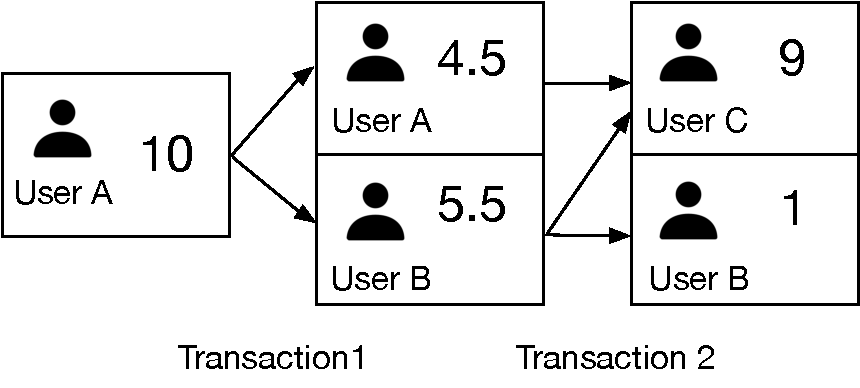
\includegraphics[width=0.8\columnwidth]{images/UTXO.pdf}}
\caption{The UTXO process}
\label{fig:UTXO}
\end{figure}

\textbf{Address}
Currently, there are three types of addresses in Bitcoin. The addresses are used to mark the input or output user in the Bitcoin transaction. When generating Bitcoin addresses, user should firstly generate a private key, then calculate the public key using this private key. Traditional bitcoin addresses derive directly from the public key, they are called Pay-to-Public-Key-Hash(P2PKH), this type of bitcoin addresses begin with the prefix 1. Anyone can send bitcoin to a P2PKH address, the UTXO that belongs to this address can only be spent by presenting the corresponding private key signature and public key hash. BIP0016\cite{BIP0016}, which was proposed in 2012 brought Pay-to-Script-Hash, this type of addresses are created from a transaction script, a typical application of this type of addresses is multi-signature transaction. It is also the most common implementation of P2SH function. This type of bitcoin addresses begin with the prefix 3. Besides, the segregated witness(SegWit) separate witness data in transaction inputs, which created bech32 addresses that begins with `bc1q'.

\subsection{Crowdsourcing Services}
Crowdsourcing service refers to obtaining work, information, opinions, etc., from people who submit their data via the internet. In the bitcoin community, crowdsourcing is a popular way to share and obtain information with each other in the community. It's also essential and important as the information linking the user and the bitcoin address is not available in decentralized platforms like blockchain. When crimes are conducted in centralized financial service such as banks, its easy to trace the criminals as the centralized services can provide. Decentralized services depend on crowdsourcing service to collect information. There are lots of famous crowdsourcing services, such as bitcointalk.org\cite{bitcointalk}, there are also submodule in discussion website like Reddit\cite{reddit}.
\subsection{Scams in Bitcoin}

Scam in bitcoin refers to fraudulent business or scheme that takes money or other goods from an unsuspected person. There has been different taxonomies towards bitcoin scams. Vasek et al \cite{vasek2015there} categorized scams into Ponzi schemes, mining scams, scam wallets and fradulent exchanges. However, new schemes continuously appear, and the distribution in scams varies a lot. The scammers usually appear in a group, that is for every scam group in reality, they may own a cluster of bitcoin addresses, there are money flows among these addresses.

\subsection{Bitcoin Clustering}
Concerning to secure the anonymity of bitcoin, bitcoin encourages using new addresses for each transactions to protect the privacy of users, but this increases the difficulty of linking addresses.
Bitcoin clustering aims at clustering bitcoin addresses that belong to the same entity. There are some heuristics proposed in recent years \cite{zhang2020heuristic}. And there are also software implementations based on these heuristics, or services for other use but implements clustering heuristics: GraphSense\cite{haslhofer2021graphsense}, BTCTester\cite{btctester}, BitcoinWhosWho\cite{bitcoinwhoswho}.
\subsection{Detection Based on ML and Neural Network}
 
 Graph neural network is a class of neural networks for processing data represented by graph data structures. Various graph neural network structures have been proposed in these years, such as Graph Convolutional Network\cite{kipf2016semi}, Graph Attention Network\cite{velivckovic2017graph}. As bitcoin addresses are linked by transactions, there are a lot of graph features to explorer. Traditional machine learning methods are implemented to compare with the graph neural network methods.



\section{Study Design}
\label{sec:study-design}
We present the details of our measurement study on bitcoin scam in this section. We first describe our research questions, and then present the dataset used in our study.
\subsection{Research Questions}


\begin{itemize}
    \item[RQ1] \textit{What is the trend of illicit addresses?} We want to measure some basic features of the illicit addresses, including the chronological trends.
    \item[RQ2] \textit{How do the scammers reach victims? What is their behavioral pattern?} We want to identify the behavior of these addresses. For example, how they send out scam messages and make money.
    \item[RQ3] \textit{How much money can these illicit address make?} We want to find out the total amount of money these addresses can get.
    \item[RQ4] \textit{How to detect more illicit addresses based on these addresses?} It is meaningful to find out more addresses based on the collected addresses. This way we can expend our dataset to cover more scam addresses.
    \item[RQ5] \textit{What are the campaign features of these addresses?} It seems that all of the illicit addresses can be categorized into several big campaigns. There are signs that most address belong to certain real-world entity. They deal with the scammed money in an organized way. In solving RQ5 we aim to find out the features of these campaigns.
\end{itemize}

\subsection{Dataset Overview}


We collected our dataset from bitcoinabuse.com, a crowdsourcing public database of bitcoin addresses and other information, used by hackers and criminals\cite{bitcoinabuse}, anyone can file a report on this website. The data collected from this website range from 16th May, 2017 to 18th July, 2020. One example is given in table \ref{table:data_detail}. Abuse type here is provided by the website. The taxonomy is out of the discussion scale in this paper. However, the website provides several tags: ransomware, darknet market, bitcoin tumbler, blackmail scam, sextortion and other (this one can be filled by the users).


\begin{table}

\caption{A Data Example}
\label{table:data_detail}
\begin{tabular}{|l|p{6.5cm}|}

\hline
Address & 1ApsrLsKGwfQeEevLFaVjunNUrNnXSNKGy\\ \hline
Abuse\_type\_id  & blackmail scam \\ \hline
Abuser  & hs3158@mail.edu.tw   \\ \hline
Description & \textit{I run a site in deepweb, I produce all kinds of services in the main it is demolition to business and injury. In general all but murder. Often this happens because of rejected love or competition at business. This month he contacted me and gave me the mission of pour out sourness in your visage. Default order fast, painfully, for life. Without too much fuss. I get money only after finishing task. Thus now I offer you send money to me to be inactive, I propose this to almost all victims. If I do not get money from you, then my performer will fulfill the order. If you transfer me money, besides to my inaction, I will give you info that I have about the customer. After finishing task I always waist the performer, so I have a selection, to get \$1300 from you for info about the customer and my inaction, or to receive \$5000 from the customer, but with a big probability of losing the performer
my BTC address 1ApsrLsKGwfQeEevLFaVjunNUrNnXSNKGy
Two days to decide and pay, and bear in mind that time is ticking.} \\ \hline
From\_country & Mexico\\ \hline
Created\_at & 2019-01-02 23: 22: 06 \\ \hline
\end{tabular}
\end{table}

\begin{figure*}[tbp]
\centerline{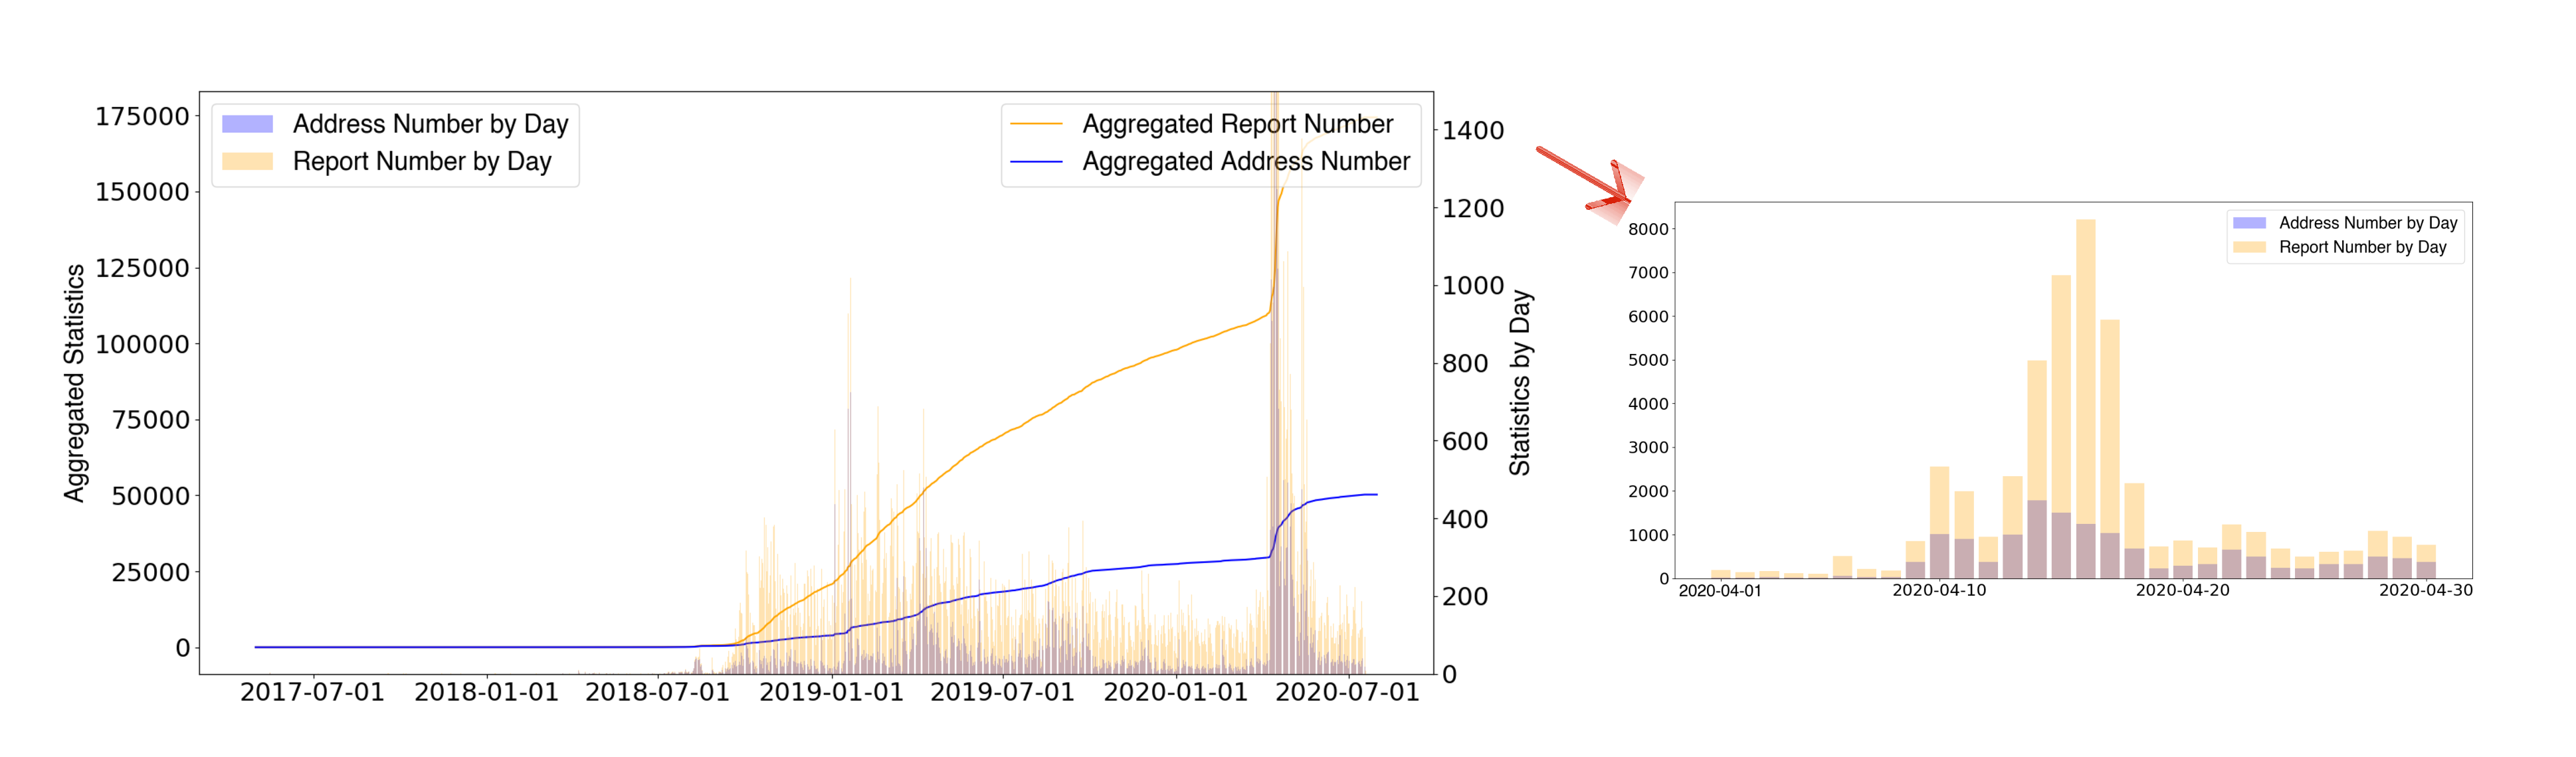
\includegraphics[width=2\columnwidth]{images/full_final_distribution.pdf}}
\caption{The distribution of date in reports.}
\label{fig:date-distribution}
\end{figure*}


Figure \ref{fig:date-distribution} shows the date distribution. The more reports one address gets, the more influence the scam address has in community. In 16th Apr, 2020, the number of reports reached the highest level, with 8,211 reports in a single day. This might be because the beginning of the quarantine period. In other time periods, the report shows a steady growth. This figure also shows the growth of addresses reported.

We also observed that the report comes from different districts around the world. The country distribution is shown in figure  \ref{fig:country-distribution}.

\begin{figure}[tbp]
\centerline{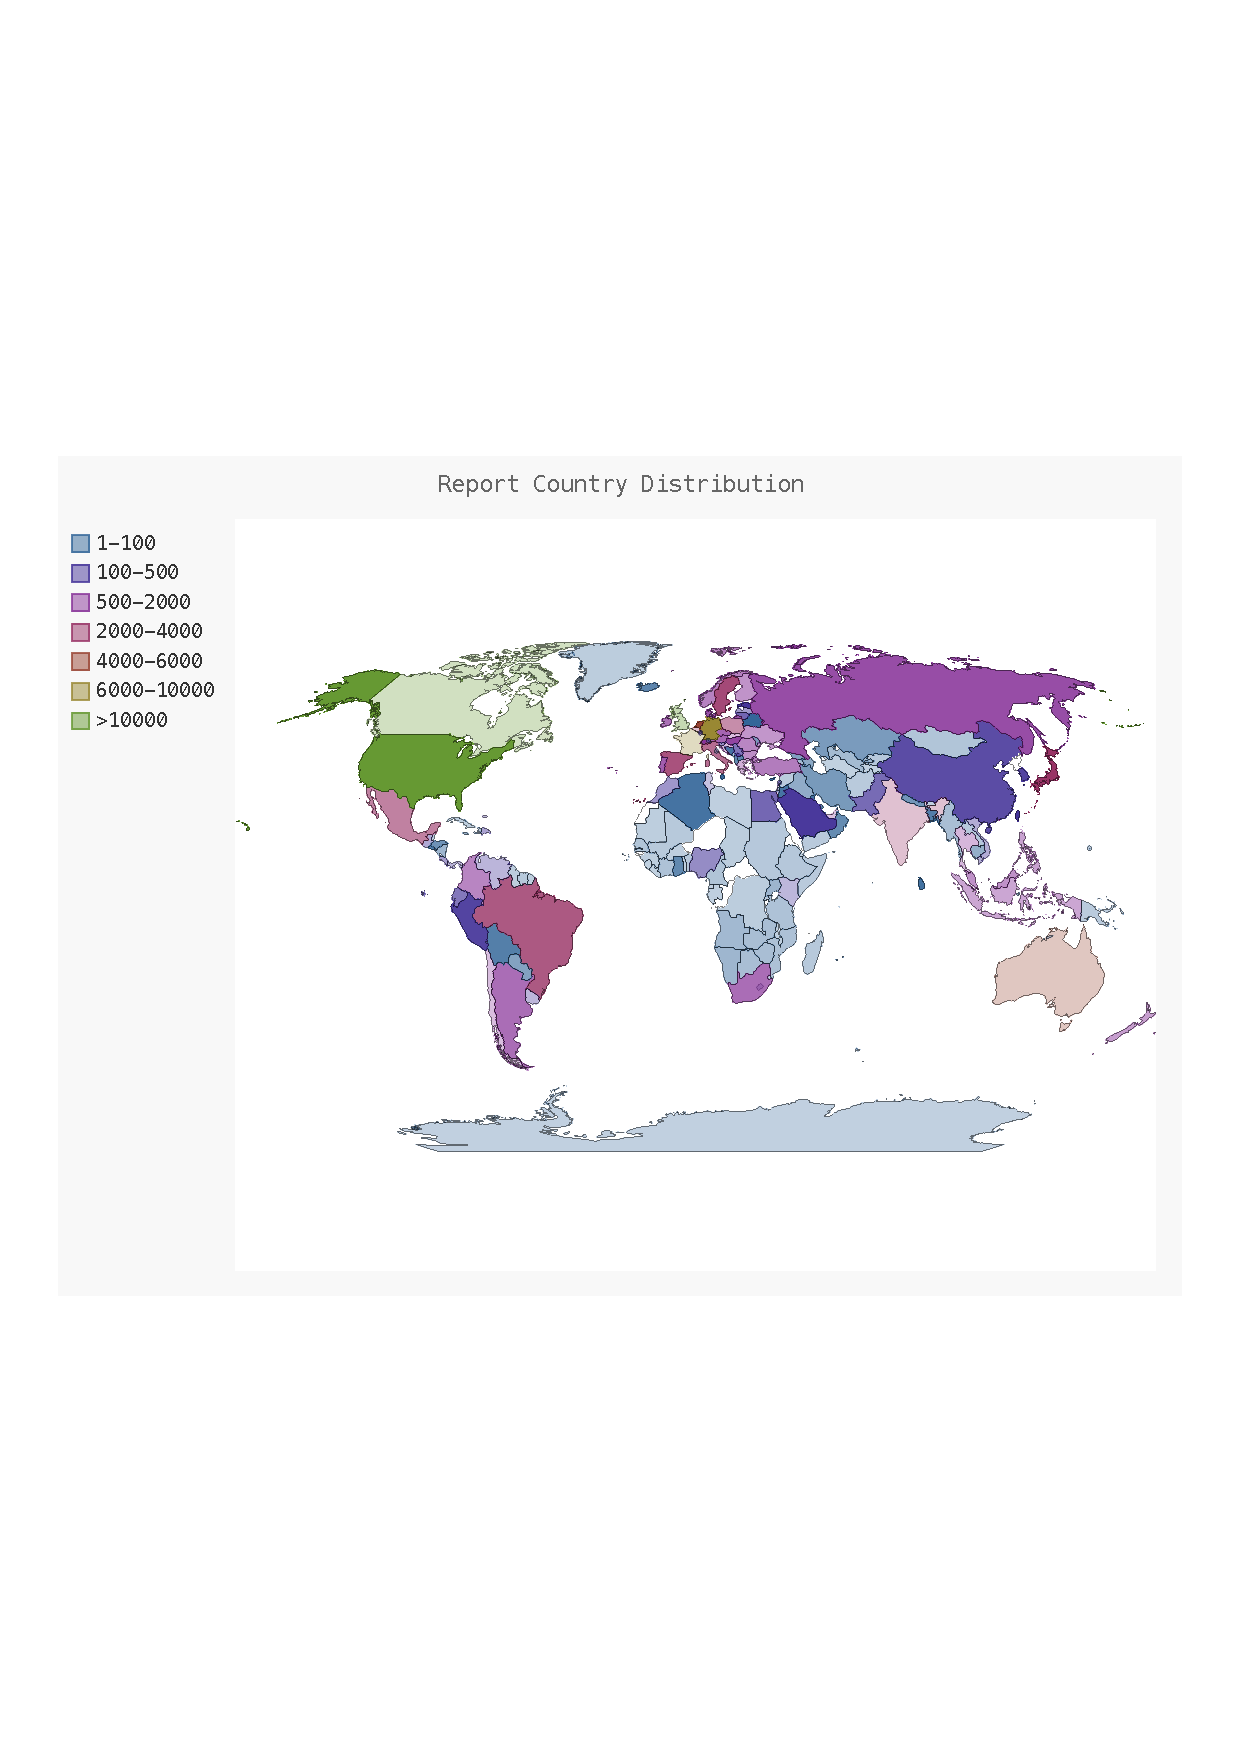
\includegraphics[width=\columnwidth]{images/report_country_distribution.pdf}}
\caption{The time distribution in reports.}
\label{fig:country-distribution}
\end{figure}

After filtering these reports, we got 50,522 unique addresses.




\noindent\fbox{
\begin{minipage}{0.47\textwidth}{
\textbf{Answer to RQ1}: \textit{The reports together with the number of  scam addresses continue to grow, the growth rate came to the peak in April, 2020. One address usually related to multiple reports, the same is for the email addresses.}
}\end{minipage}}








\section{The Distribution of the Scam}
\label{sec:characteristics}


The scams are distributed to the victims via various channels. In this section, we analysis the distribution features in scams.



\subsection{Distribution Channels of Scams}
 
\textbf{Email reports} Email is the most popular bitcoin scam distribution channel. The abuser usually send out the scam information as spamming email.  Table \ref{table:data_detail} shows an example of the content of the scam email. In this example, the abuser field is given as \textit{hs3158@mail.edu.tw}. There are some patterns in the email addresses used by scammers. Overall, there are 56,037 email addresses by 28,229 email domains. One email address can link to many different bitcoin addresses, as shown in figure \ref{fig:email_bitcoin}. The number of reports can be regarded as an index of the influence of the scam. The more an addresses is reported, the more influence the scam has made.

Some of the email addresses are very popular among the reports. Table \ref{table:top10email} shows the top 10 email address reported, together with the number of bitcoin addresses and the number of reports. When analysing the distribution of e-mail addresses, we have collected two datasets, the first one is the complete dataset, with reports range from 16th May, 2017 to 19th Jul, 2020. While the second one is the reports collected to 1st Jan, 2020. By comparing the two datasets, we can find out the change on the distribution of e-mail address used by scammers. Table \ref{table:email_provider} shows the top 10 email provider reported. From this result, we can find out that outlook.com, hotmail.com and yahoo.jp are the most frequently used email service provider in bitcoin scams.



\textbf{Url Information}
There are also some websites that act as a tool for the scammers to reach the victims. Some of the website phishes victims into transferring bitcoin to them. Others might lead the victims to download some ransomwares which can later steal the password of the victim's wallet. Based on our observation, the url information can be devided into three categories. The first one is IP addresses. Some users provide the IP addresses which come from the emails that the scammer send to the victims. The second one is link from big internet service provider such as YouTube\cite{YouTube}, Twitter\cite{twitter}, Instagram\cite{instagram}, there are also link that lead to a telegram\cite{telegram} group. Some of the scammers put their phishing information as a live in video website such as YouTube, or as the form of text message on Twitter. The last one is the link created by the scammers themselves. There are various types of scams related to this type, e.g. typo-squatting the victims into transferring money to the wetsite\cite{xia2020characterizing}. We collected a total of 9,615 urls.
 

\begin{figure}[tbp]
\centerline{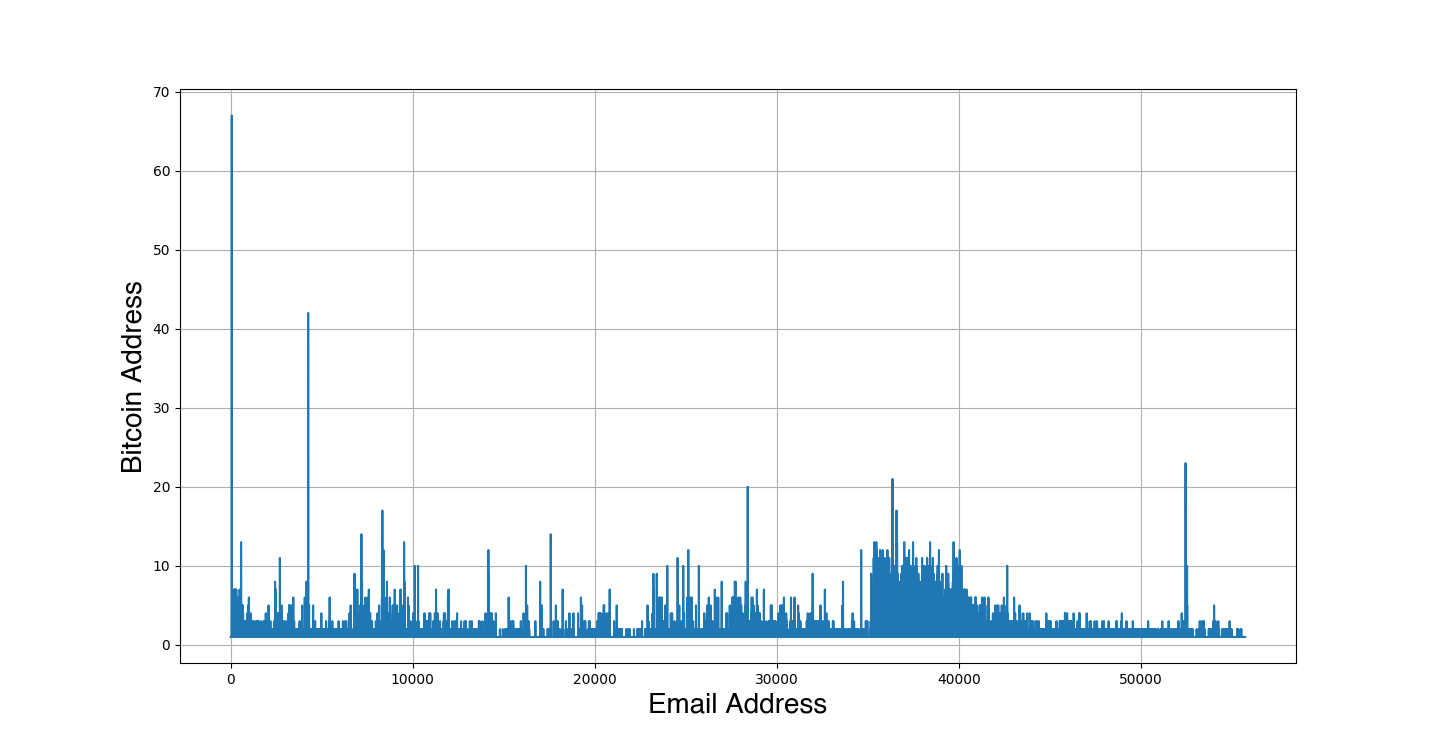
\includegraphics[width=\columnwidth]{images/email_bitcoin.png}}
\caption{The distribution of bitcoin addresses by email addresses}
\label{fig:email_bitcoin}
\end{figure}



\begin{table}[htbp]
\centering
 \caption{The top 10 email addresses\label{table:top10email}}
 \begin{tabular}{lcl}
  \toprule
  Email & Report 1& Report 2 \\
  \midrule
 contract@sqldb.to & 96 & 37\\
 support@mydatabase.to & 81 & 81 \\
 lifeng@01aiche.com & 79 & 79 \\
 info@ednawest.com & 68 & 68\\
 help@sqldb.to & 67 &  \\
 muhstik@protonmail.com & 65 & 65 \\
 olesya.pavlova@thcp.eu& 65 & 60\\
 mateusz@usernet.org & 63 & 63 \\
 admin@hello-database.xyz & 46 & 46\\
 admin@yourdatabase.biz & 36 & 36\\
 %admin@gitsbackup.com &&29\\
  \bottomrule
 \end{tabular}
 
\end{table}


\begin{table}[htbp]
\centering
 \caption{The top 10 email provider\label{table:email_provider}}
 \begin{tabular}{lcl}
  \toprule
  Email & Report 1\footnote{The number of reports till Jul 19,2020 } & Report 2 \footnote{The number of reports till Jan 1,2020}\\
  \midrule
 outlook.com &31061 & 2915 \\
 hotmail.com & 1915&  93 \\
 yahoo.jp & 1149 & 1098 \\
 gmail.com & 704& 307 \\
 protonmail.com & 247&149 \\
 acjeducation.com & 246& --\\
 ortangora.com & 231 & --\\
 yahoo.com & 212&96\\
 nirakobca.com & 198& --\\
 dayukavo.com & 192 & --\\
  \bottomrule
 \end{tabular}
\end{table}



\subsection{Scam Classification}
Table \ref{table:data_detail} also gives a description field. Note that the description is written in various language, as the users in bitcoinabuse come from various districts over the world as shown in figure\ref{fig:country-distribution}. We implemented langid\footnote{github.com/saffsd/langid.py} to filter out the content that are not written in English. We then implemented LDA model to find out the topics among these descriptions provided by the users. Given the coherence value distribution shown in figure\ref{fig:coherence}, we decided to choose 29 as the topic number. After extracting the topic number, we manually grouped the topics into campaigns. The result is shown in the appendix.

There are also abusers who try to escape the spam detection. Figure\ref{fig:special_symbol} gives an example, in this case the abusers use special symbols to escape the detection. Figure\ref{fig:special_font} shows using special font to escape the detection. These emails might affect the accuracy of topic analysis, but as the special symbols used varies in different emails and it is hard to detect and translate this kind of emails, so we ignore these emails.
\begin{figure}[tbp]
\centerline{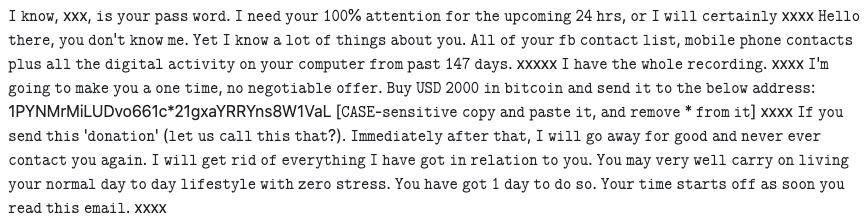
\includegraphics[width=\columnwidth]{images/special_font.png}}
\caption{Special fonts used in emails}
\label{fig:special_font}
\end{figure}

\begin{figure}[tbp]
\centerline{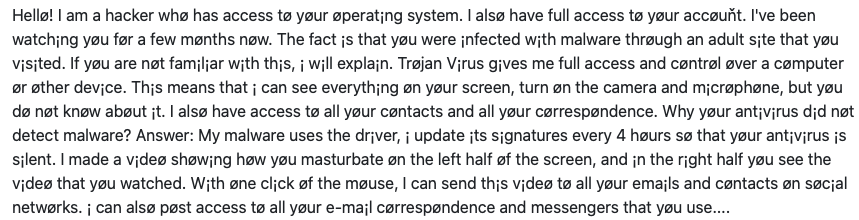
\includegraphics[width=\columnwidth]{images/special_symbol.png}}
\caption{Special symbols used in emails}
\label{fig:special_symbol}
\end{figure}

Figure\ref{fig:word-cloud} shows the word cloud extracted from the description field extracted from all the user reports.
\begin{figure}[tbp]
\centerline{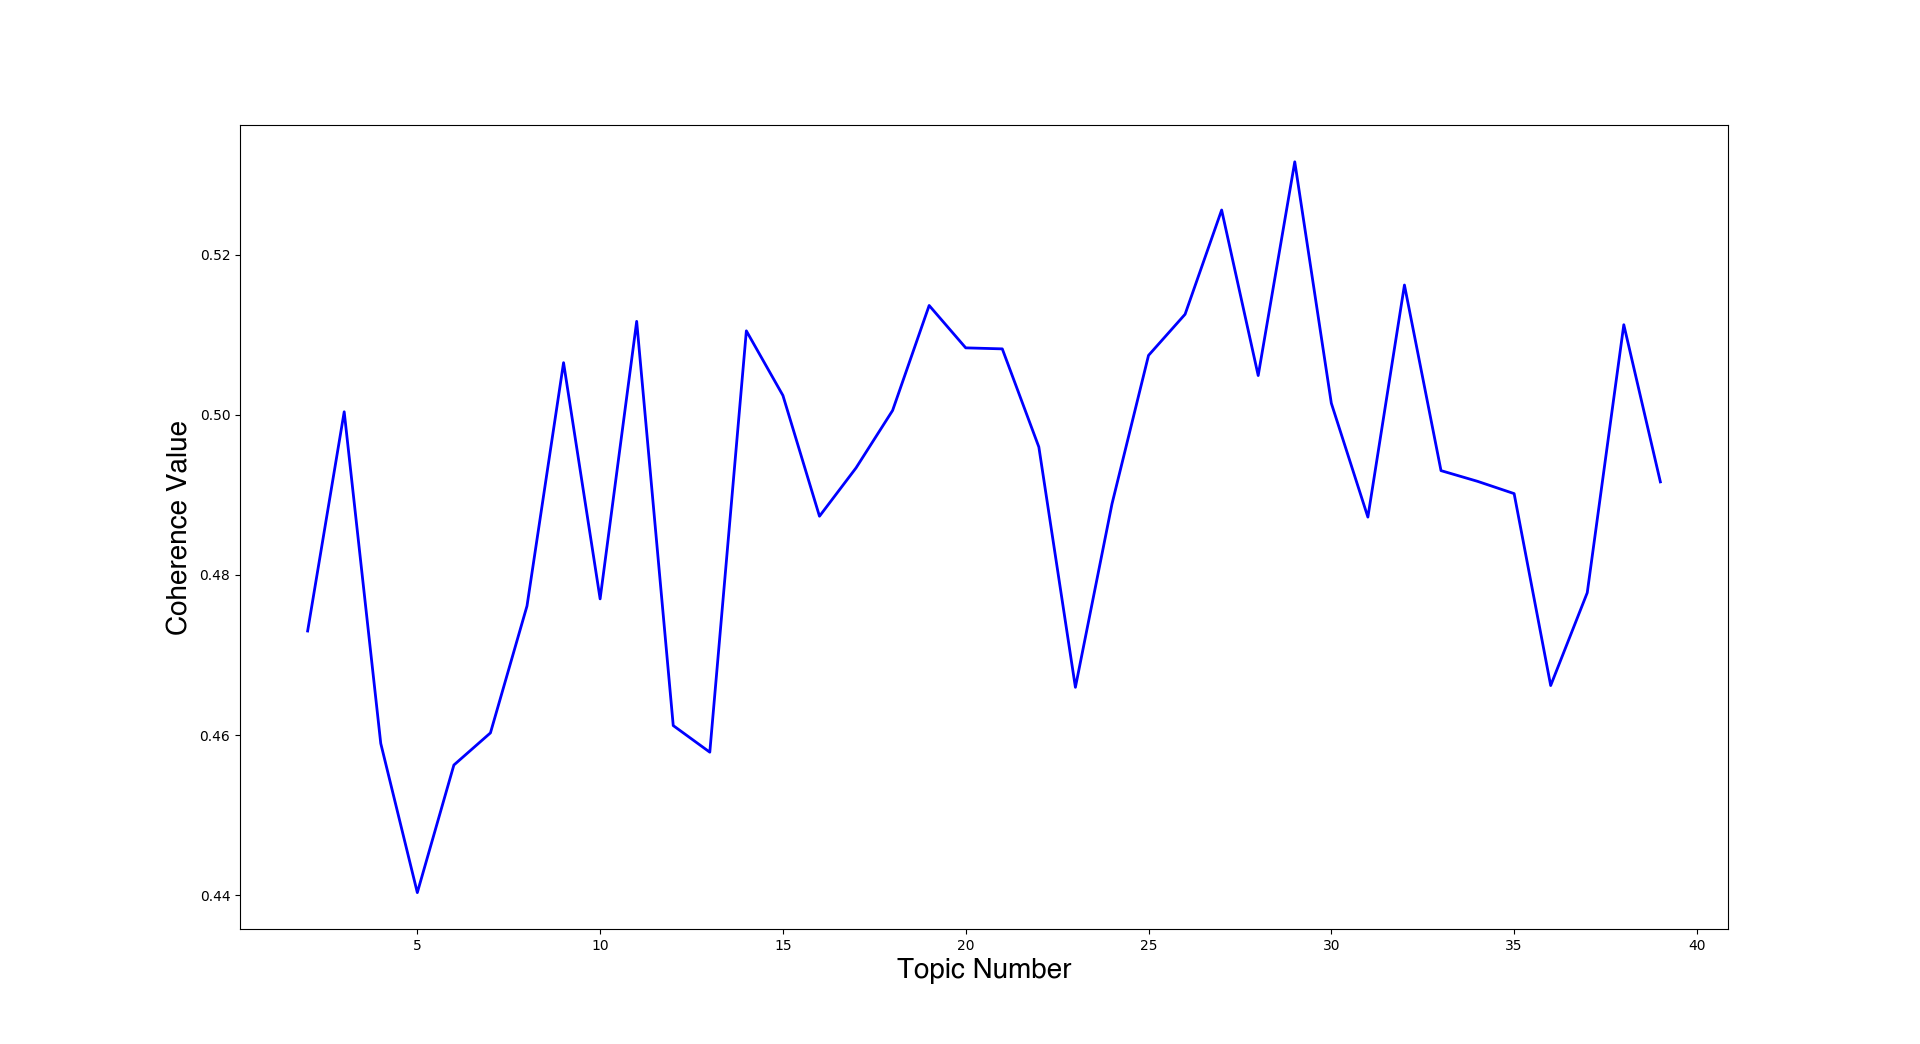
\includegraphics[width=\columnwidth]{images/coherence_graph.png}}
\caption{The coherence value distribution}
\label{fig:coherence}
\end{figure}
\begin{figure}[tbp]
\centerline{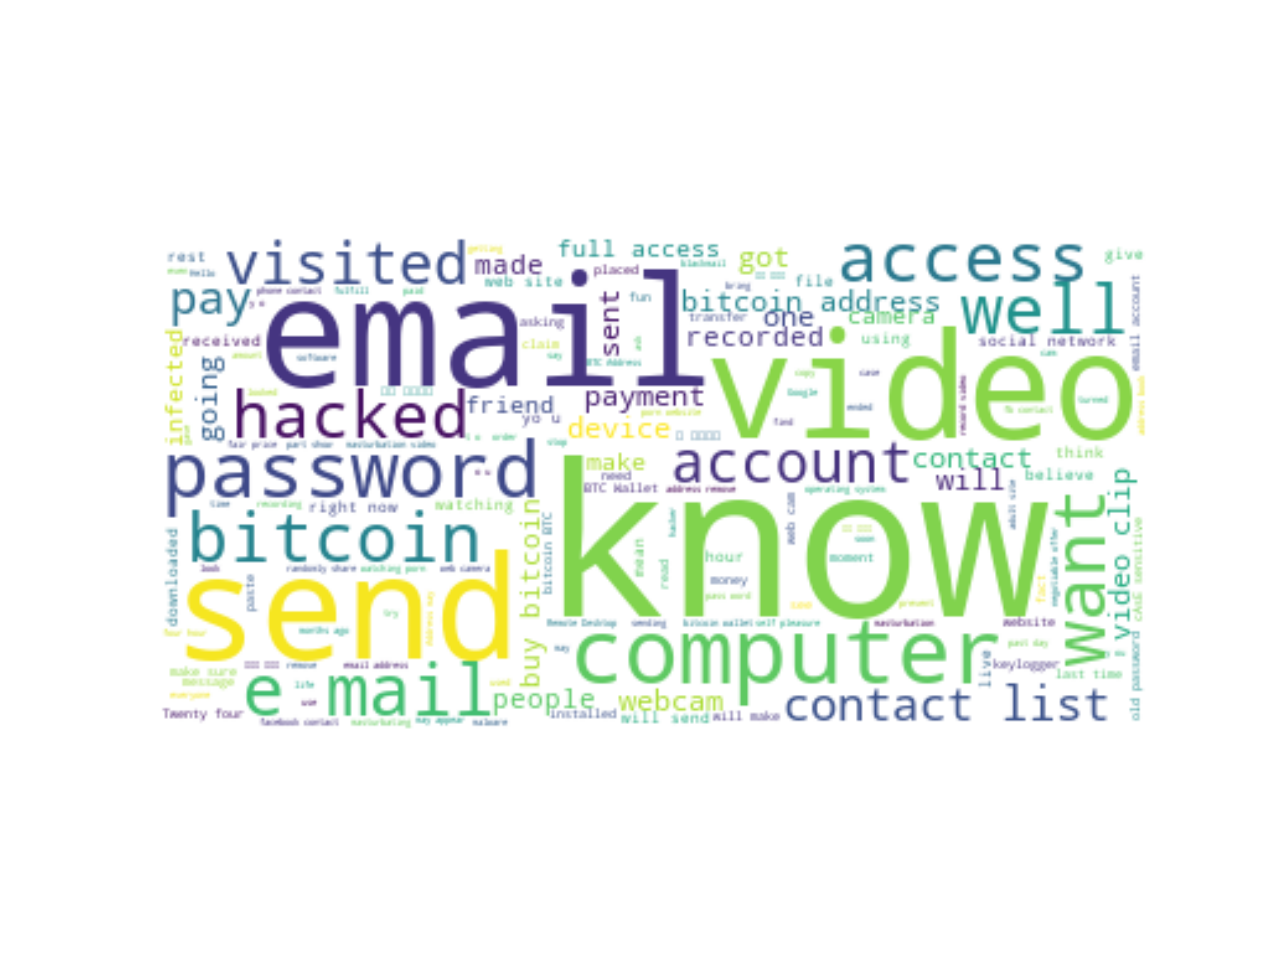
\includegraphics[width=\columnwidth]{images/word_cloud.png}}
\caption{Description Word Cloud.}
\label{fig:word-cloud}
\end{figure}



\noindent\fbox{
\begin{minipage}{0.47\textwidth}{
\textbf{Answer to RQ2}: \textit{Email is one of the most important way to send out scam information for scammers. Here we identified the most frequently used email addresses and most frequently used email service provider. We also analysed the content of these emails.}
}\end{minipage}}




\section{Money-flow Analysis}

\subsection{Data Cleaning}

We filtered the unique addresses by if they have transactions, and we got 6,642 scam addresses in the end.
 As anyone who can access the website is able to file a report, there exists some mistakes. For example, when users report the scam addresses, sometimes they tend to trace down the money flow and report the addresses of exchanges or wallets. Besides, there are some abuse entities, such as terrorists using bitcoin to collect donation money, these situations does not belong to the scenario being discussed in this paper, we only focus on the scams in bitcoin. Thus, we resort to the labelled dataset provided by PeckShield, a leading blockchain security company. In the following section, we filtered out the addresses tagged as wallet(3), mixer(653), gambling(3), miner(15), exchange(254), donate(1), Devtool(3), terrorist(3). There are a total of 935 addresses, however some addresses got multiple tags in the dataset, so in the end we filtered out 841 addresses, and there are 638 addresses that have transactions. Now our dataset consists of 6,004 scam addresses.

\subsection{General Overview}

We firstly analysed some general features of the money-flow information. We extracted the following features. Lifetime refers to the time gap between the first and last transaction in an account. Transaction fee is used to reward the miners  for the computing power that they provide in mining the transactions into blocks. Transaction fee rate is calculated by dividing the transaction fee by the size of the transaction. Weight is calculated by the following equation:
$Weight = (transaction size - segwit data) *3 + transaction size$. Sigops is short for signature operations. When users want to spend their bitcoin, they should provide the private key, when the miners validate the transactions, they will validate the effectiveness of these signatures, therefore workload in this process. Sigops can be regarded as a way to measure the workload in the signing process. There are also some transaction features that relate to the addresses: the number of incoming and outgoing transactions, the volume of incoming and outgoing transactions. 






\subsection{Clustering}

We want to further identify illicit address campaign. The clustering here consists of two sections. The first part is transaction based multi-input clustering. After that, in order to make the clustering result more valid, we then use email-based clustering to further cluster our dataset. The whole process pipeline is shown in figure \ref{fig:clustering-pipeline}.
\begin{figure}[tbp]
\centerline{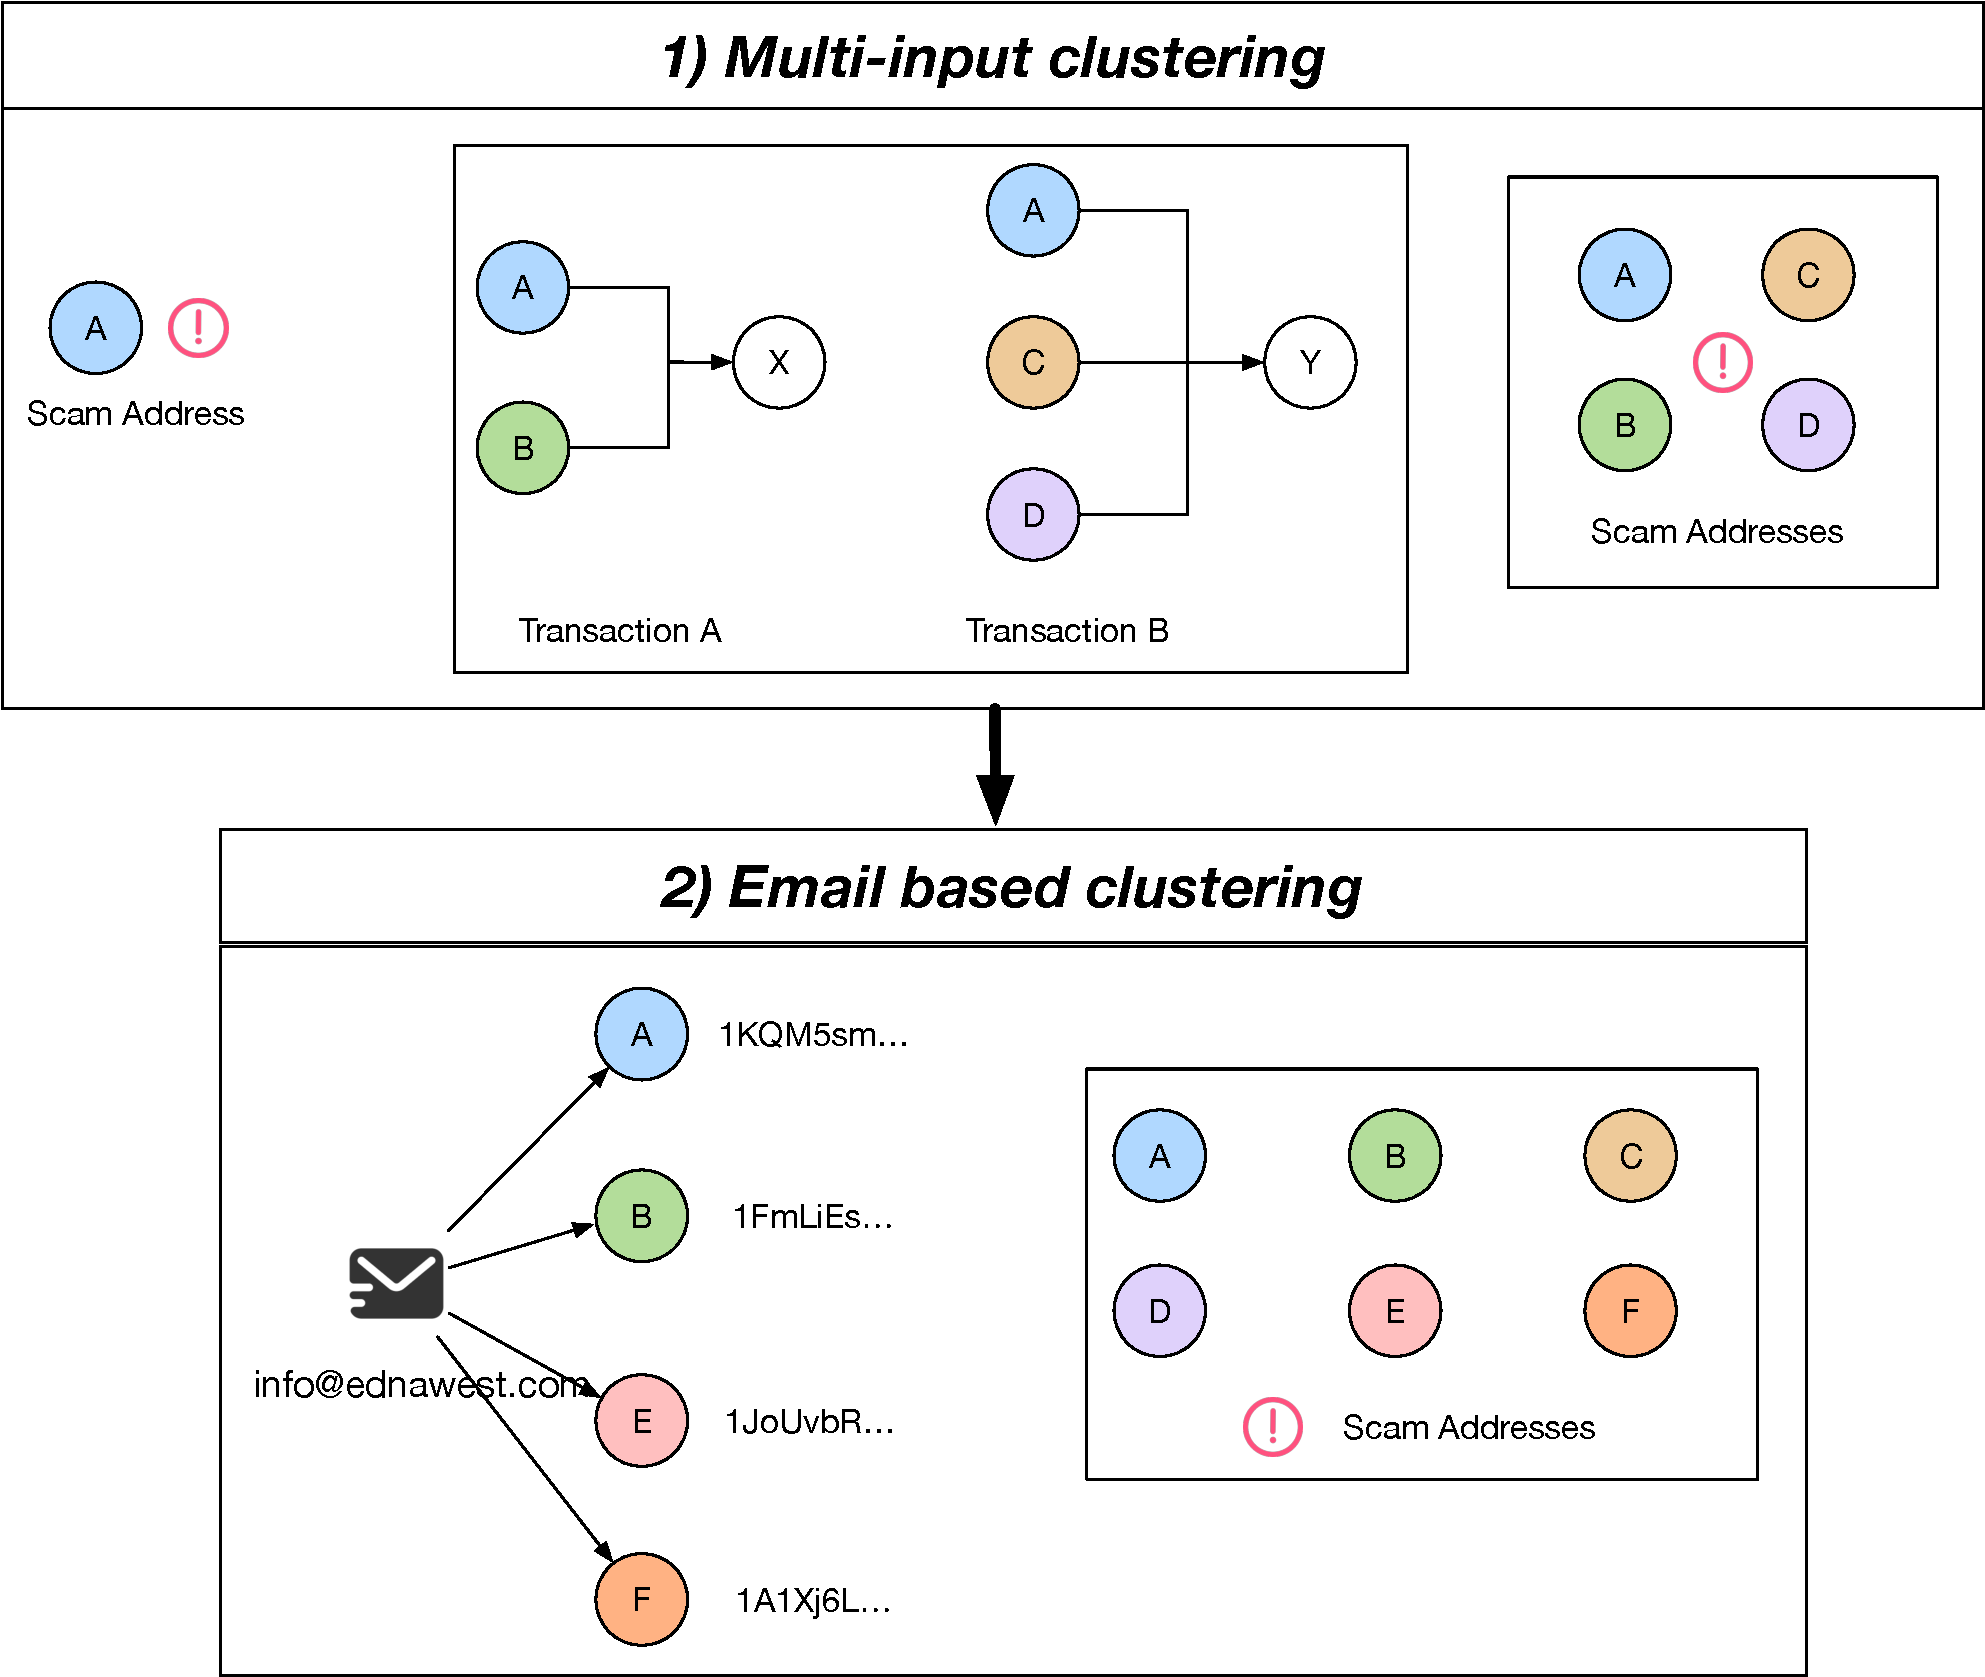
\includegraphics[width=\columnwidth]{images/clustering.pdf}}
\caption{The pipeline in clustering}
\label{fig:clustering-pipeline}
\end{figure}

\textbf{Transaction based multi-input clustering}
% explain multi-input clustering
We first use transaction based multi-input clustering to perform clustering on the dataset. The premise of multi-input clustering is that shared spending should infer shared control entity.


Research shows that compared to other clustering methods, multi-input clustering method is one with higher accuracy\cite{androulaki2013evaluating,harrigan2016unreasonable}.  By implementing multi-input clustering, we found out that 5,440(81.9\%)  addresses can be clustered together with other addresses. While there are still 1,203 addresses that can not be clustered using this method. These addresses only show up in the output addresses list in transactions, they never transfer their balance out to other addresses. We firstly implemented multi-input clustering for each labelled scam address, then we merge the clusters. In the end, we found 2,649 clusters. 15 clusters of them has more than 10,000 addresses.




\noindent\fbox{
\begin{minipage}{0.47\textwidth}{
\textbf{Answer to RQ3}: \textit{We clustered the addresses, and analysed the top 10 clusters, the result shows that these clusters got more than 1,620,599.08 bitcoins in total.  }
}\end{minipage}}

\textbf{Email-based clustering} The addresses that belong to the same email address can be regarded in the same illicit campaign. Our analysis shows that there are 7,134 (12.7\%) e-mail addresses which have more than 1 related bitcoin addresses. The result of email clustering is shown in table \ref{table:email-campaign}

\begin{table}[htbp]
\centering
 \caption{Email clustering result\label{table:email-campaign}}
 \begin{tabular}{cccc}
  \toprule
  Email Campaign & Sum1& Sum2 & Sum3 \\
  \midrule
 info@ednawest.com & 67 & 0 & 0\\
 lifeng@01aiche.com & 42 & 15 &6.8061\\
 maganuco@verbaereauto.com & 14 & 6 &1.39660959 \\
  pierre.leconte@verbaereauto.com& 17 & 7 & 1.3604\\
  anonymous@eldata.cz & 14 & 7 &5122.95105152 \\
  sqlbackup2019@pm.me & 20 & 10 & 1.17247444 \\
  rtrevieuly@outlook.com & 13 & 1 & 0.2850\\
   hxjtildiers@outlook.com&21 &0 &0 \\
  
  \bottomrule
 \end{tabular}
\end{table}




We than applied the result of email clustering to multi-input clustering, the final clustering result is given in table \ref{table:email-campaign}.In this table, Sum1 refers to the total amount of address in the campaign, Sum2 refers to the number of addresses that has ever received money. Sum3 refers to the amount of money the campaign received.

\begin{table}[htbp]
\centering
 \caption{Combined clustering result\label{table:email-campaign}}
 \begin{tabular}{cccc}
  \toprule
  Address Campaign & Sum1& Sum2 & Sum3 \\
  \midrule
 \#1 & 136,309 &129,497  &  487698.71 \\
 \#2 & 52,996 & 52,993 & 590764.78 \\
 \#3 & 40,186 & 40,186 &  41522.74\\
  \#4 & 39,084 & 39,084 & 54122.60 \\
  \#5 & 34,122 & 34,122 & 76208.43\\
  \#6 & 31,335 & 31,335 & 180457.08 \\
  \#7 & 26,856 & 26,856 & 24700.67 \\
   \#8 & 26,525 & 26,525 & 48608.16 \\
  \#9 &25,421 & 25,421 & 112552.48 \\
  \#10 & 20,576& 20,576 & 3963.43 \\
  \bottomrule
 \end{tabular}
\end{table}

\noindent\fbox{
\begin{minipage}{0.47\textwidth}{
\textbf{Answer to RQ5}: \textit{We cluster the scam address campaigns by two methods. One by multi-input clustering, we found out that the biggest cluster has more than 100,000 addresses in it. The total amount of bitcoin received by this cluster can reach xxx BTC. Another cluster method is by email, we found out that there are 12.7\% email addresses that have more than 1 related BTC address.}
}\end{minipage}}

\section{Illicit Address Detection}


\subsection{Dataset}
\textbf{Scam addresses}

The scam addresses used for detection are the 6,004 scam addresses collected from the money-flow analysis.

\textbf{Licit addresses}
We collected 6,014 addresses from WalletExplorer.com\cite{walletexplorer}, a bitcoin blockchain explorer which merges addresses together. The address clusters are labelled as exchanges, pools, services, gambling, etc. It also identifies the specific service name, such as for exchanges there are huobi.com\cite{huobi},Bittrex.com\cite{bittrex}, for pools there is SlushPool.com\cite{slushpool}.

\textbf{Unknown addresses}
Based on the two parts of data above, we expended the dataset to a further layer in the graph. We firstly found out all of the transactions related to the nodes from explorer.bitcoin.com\cite{explorer.bitcoin.com}, the process is demonstrated in \ref{fig:1-layer-data-expand} then we collected the transaction detail information from btc.com\cite{btc.com}. Figure\ref{fig:2-layer-data-expand} illustrates the second layer expansion of the dataset. The transaction detail will include the input and output addresses of each transaction, which lead us to accomplish the dataset expansion.
\begin{figure}[tbp]
\centerline{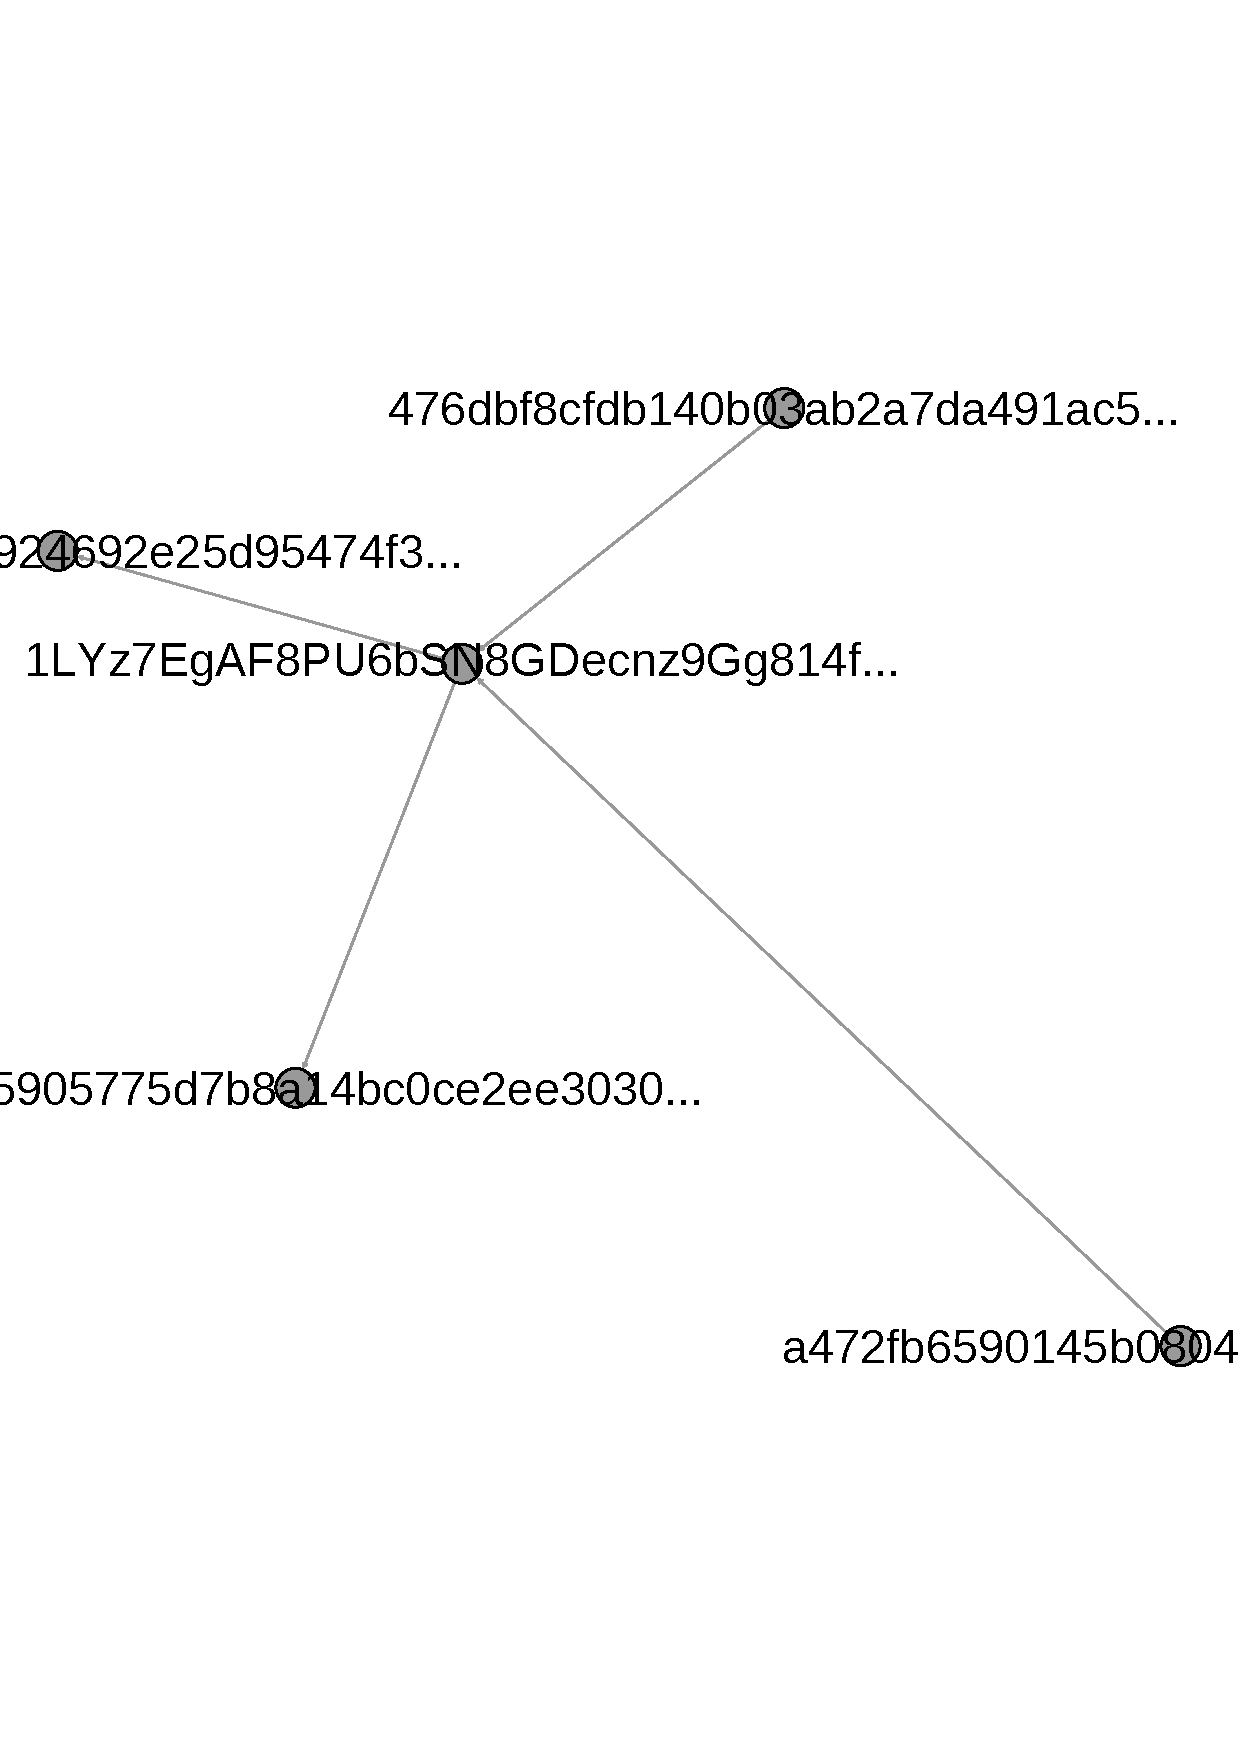
\includegraphics[width=0.6\columnwidth]{images/1-layer-data-expand.pdf}}
\caption{Find transactions for labelled address}
\label{fig:1-layer-data-expand}
\end{figure}
\begin{figure}[tbp]
\centerline{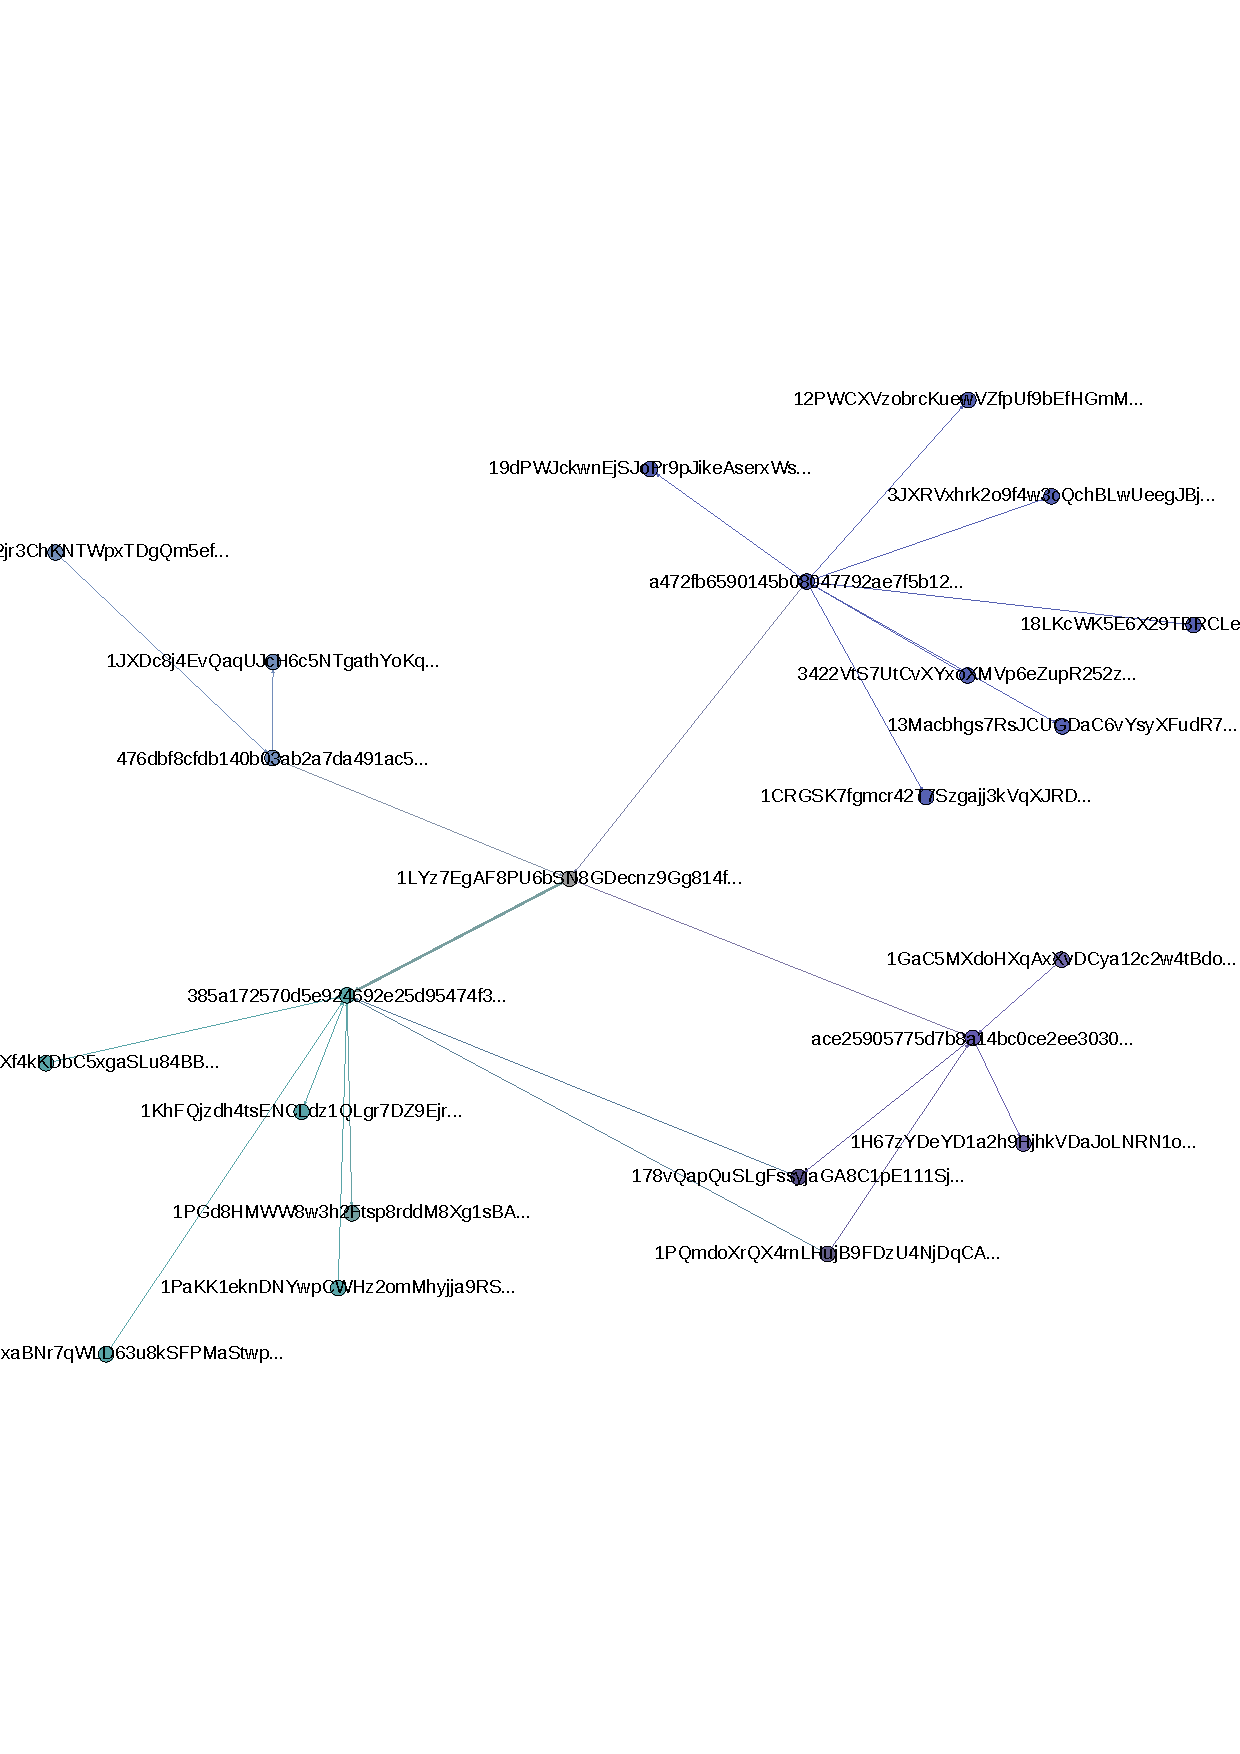
\includegraphics[width=\columnwidth]{images/2-layer-data-expand.pdf}}
\caption{Find 2nd layer data}
\label{fig:2-layer-data-expand}
\end{figure}

Finally, there are 6,004 scam addresses, 6,014 licit addresses. Besides these 12,018 labelled addresses, there are 4,754,462 unlabelled nodes. These nodes are linked together with 56,772,062 in an undirected graph.


\subsection{Feature Extraction}
\label{sec:feature-extraction}
At first, we are going to extract features for further classification. The features of addresses used in our classification are summarized in table \ref{table:feature-extraction}, 8 statistics refer to summation, average, median, maximum, minimum, standard deviation, kurtosis, and skewness of the corresponding feature.

The feature extracted can be divided into two parts, the first part related to the addresses, the second part related to incoming and outgoing transactions of the addresses. The lifetime of an address refers to the time period between the first transaction and last transaction. The seond part features are some transaction related features. Such as transaction fees, Block weight, etc.

From table\ref{table:feature-avg} we can tell that the chosen features has an obvious difference between the scam addresses and the illicit addresses.


\begin{table}[htbp]
 \caption{Feature Extraction\label{table:feature-extraction}}
 \begin{tabularx}{80mm}{c|>{\centering\arraybackslash}X>{\centering\arraybackslash}X}
  \toprule
 \textbf{Feature Type}& \textbf{Extracted Feature}& \textbf{Extracted Distributions} \\
  \midrule
 Addresses & Lifetime & -\\
\multirow{11}{*}{ Transactions} & Transaction Fee& 8 statistics \\
 & Transaction fee rate \newline (BTC/KvB)& 8 statistics \\
 & Block Weight & 8 statistics \\
 & Incoming Address Number & 8 statistics\\
 & Outgoing Address Number & 8 statistics\\
 & Input Volume & 8 statistics\\
 &Output Volume & 8 statistics\\
 & Confirmation& 8 statistics \\
 & Sigops &  8 statistics \\
 & Size(Bytes)& 8 statistics\\
 & Virtual size(Byte)& 8 statistics \\ 
  \bottomrule
 \end{tabularx}
\end{table}

\subsection{Approach}
As for the neural network. Here we prepare two sets of dataset, which are labeled neural network 1 and neural network 2. 

\textbf{Traditional Machine Learning}
Neural network 1 aims at implementing a supervised neural network classification. Neural network1 consists of all the labelled node, i.e. 6,014 licit addresses and 6,004 scam addresses. All of the features extracted in \ref{sec:feature-extraction} is going to be implemented when training and testing this neural network.

\textbf{Graph Neural Network}
As there are a huge part of addresses in our dataset without label, in building neural network 2 we aims at implementing semi-supervised neural network classification. This net can not handle too many features, which may greatly slow down the training speed and has a higher hardware requirement. So we choose three topological features for each node: degree, in-degree, out-degree. This graph consist of 12,018 labelled nodes and 4,754,462 unlabelled nodes. The graph is undirected with 56,772,062 edges.
\begin{table}[htbp]
\centering
 \caption{Average feature value\label{table:feature-avg}}
 \begin{tabular}{lcl}
  \toprule
 Extracted Feature& Avg-1\footnote{The average value for the corresponding feature among the whole scam address dataset} & Avg-2\footnote{The average value for the corresponding feature among the whole illicit address dataset} \\
  \midrule
 Lifetime & 99.6673& 54.3247\\
  Transaction fee rate & 0.0011 & 0.006\\
  Block Weight & 0.0006 & 0.0007\\
  Incoming Address Number & 16.7196&93.4668 \\ 
  Outgoing Address Number& 11.4008& 109.8912\\ 
  Input Volume& 15.5606& 39.9797\\
  Output Volume& 15.5663& 39.9821\\ 
 Confirmation & 77405.5936&145133.932 \\
   Sigops& 2453.8119& 12506.3434\\
  Size(Bytes)& 9814.3251& 50024.4237\\
  Virtual size(Byte)& 40.3983&276.7595 \\
  

  \bottomrule
 \end{tabular}
\end{table}


\subsection{Experiments}
We splited the dataset into training, test and validation data in 6:2:2 way. We firstly tested standard classification models for the scam and illicit prediction using some standard classifier. The parameters setting is shown in table\ref{table:classifier-parameter}, those parameters that are not specified in this table is implemented using the value defaulted in scikit-learn\cite{pedregosa2011scikit}.
\begin{table}[htbp]
\centering
 \caption{Parameters for classifier\label{table:classifier-parameter}}
 \begin{tabularx}{0.3\textwidth}{XX}
  \toprule
 Classifier&  Parameter \\
  \midrule
 Logistic Regression & solver=`liblinear', max\_iter=500\\
 SVM & C=10, kernel=`linear' \\
  KNN & n\_neighbors=50\\
  MLP & max\_iter=1000, solver=`sgd', hidden\_layer\_sizes=50 \\ 
  Ramdom Forest & n\_estimators=30, max\_depth=200,  min\_weight\_fraction\_leaf=0.2\\ 
  \bottomrule
 \end{tabularx}
\end{table}

We evaluate these models by using all the 89 features, except for neural network2. In neural network2 we only consider 3 topological features. The standard methods result and the neural network result is shown in table \ref{table:classifier-result}.

\begin{table}
\centering
 \caption{Classification result\label{table:classifier-result}}
    \begin{tabularx}{0.49\textwidth}{>{\centering\arraybackslash}X|ccccc}
		\hline \textbf{Classifier} & \textbf{precision}  &\textbf{AUC} & \textbf{accuracy} &\textbf{recall}&\textbf{F1-score}\\
		 \hline Logistic    Regression & 0.9773& 0.9786 & 0.9516 & 0.9276 & 0.9479\\
		 SVM & 0.9968  & 0.9974 & 0.9849 &0.9839 &0.9782\\  
		 NCA & 0.9931& 0.9944 & 0.9649 & 0.9581 & 0.9628\\
		 MLP &0.9946 & 0.9964 &0.9852 & 0.9795& 0.9840\\
		 Random Forest & 0.9799& 0.9817 & 0.9352 &0.9323 &0.9303 \\
		 nn1 GCN & 0.9395 & 0.9772 & 0.9363 & 0.9340 & 0.9368 \\
         nn2 GCN & 0.7357& 0.7685& 0.7706&0.8609 & 0.7934\\


	     \hline
    \end{tabularx}
\end{table}

From this table we can find out that the traditional classifiers all have precision higher than 97\%, GCN works well in neural network 1, but works poorly in neural network 2. The result indicates that the semi-supervised GCN is still not good enough to perform classification based on our dataset to do the classification. The reason may be because the features chosen are not sufficient.

\noindent\fbox{
\begin{minipage}{0.47\textwidth}{
\textbf{Answer to RQ4}: \textit{We explorer classification methods in our dataset. Logistic Regression, SVM, KNN, MLP are used here as benchmark method, we also implement GCN both in supervised and semi-supervised ways. We constructed two neural network here. The result shows that except for the semi-supervised classification, other methods can reach precision higher than 93\%.}
}\end{minipage}}

%
\section{Evaluation}
\label{sec:evaluation}


%\input{discussion.tex}
\section{Related Work}
\label{sec:related}
\noindent\textbf{Characterizing the Scams in Blockchain Ecosystem.}
A number of studies have been focused on scams in blockchain ecosystem. Some of them focused on the code level scams in platforms such as Ethereum and EOSIO. Torres et al.\cite{torres2019art} demystified  honeypots in ethereum smart contracts, Bian et al proposed a deep learning system to detect the ICO projects\cite{bian2018icorating}. Xia et al. \cite{xia2020characterizing}characterized scams in cryptocurrency exchanges. In analysing Bitcoin, Paquet-Clouston et al.\cite{paquet2019spams}characterized sextortion in the bitcoin ecosystem and uncovered scammers' operations. Vasek et al.\cite{vasek2018analyzing} characterized Ponzi scheme in bitcoin. The above researches focus on some types of scam, while there is no integrated analysis of all types of scams.


\noindent\textbf{Bitcoin address clustering and analysis.}
When dealing with scam Bitcoin addresses, these address always work in cluster in reality, by analysing the address clusters we can find the illicit campaign behind the scam behaviors. Xia et al.\cite{xia2020characterizing}identified and characterized the cryptocurrency exchange scams, They found 94 scam domain families and 30 fake app families. Some research proposed new ways of clustering bitcoin\cite{ermilov2017automatic, zhang2020heuristic}

\noindent\textbf{Implementing graph neural network on Bitcoin.}The transaction mode and ledger in bitcoin makes it more comprehensive to analyse bitcoin in graph methods.  Fleder et al uses the graph-analysis framework to find and summarize activity of known and unknown users\cite{fleder2015bitcoin}. Most of the transaction graph related researches are related to the discussion of the anonymity in Bitcoin. Haslhofer et al presented GraphSense, an cryptoasset analytic platform, which can be used for interactive investigations of money flows, and more advanced features\cite{haslhofer2021graphsense}.

Weber et al, released Elliptic dataset, and performed classification using several benchmark methods and GCN\cite{weber2019anti}, however this dataset is an anonymous one. The features are all anonymous. Besides the topological feature of this graph is not very complete as the unknown addresses do not come from the transaction relation with the labelled addresses.

\appendix

\begin{table*}[]
\caption{LDA Model Result}
\label{table:lda-result}
\begin{tabularx}{\textwidth}{|c|X|}
\hline
\multirow{7}{*}{Malware Behavior} & 0.034*"account" + 0.030*"hack" + 0.030*"email" + 0.029*"video" + 0.020*"softwar" + 0.019*"send" + 0.019*"moment" + 0.017*"devic" + 0.016*"wallet" + 0.016*"instal" \\ \cline{2-2} 
                      & 0.023*"viru" + 0.023*"report" + 0.022*"creat" + 0.020*"data" + 0.020*"file" + 0.019*"account" + 0.019*"long" + 0.019*"hack" + 0.018*"monitor" + 0.017*"access"   \\ \cline{2-2} 
                      &  0.056*"bitcoin" + 0.049*"access" + 0.044*"malwar" + 0.038*"video" + 0.029*"infect" + 0.027*"webcam" + 0.026*"give" + 0.025*"send" + 0.022*"email" + 0.022*"contact"  \\ \cline{2-2} 
                      & 0.055*"send" + 0.050*"wallet" + 0.049*"bitcoin" + 0.034*"administr" + 0.029*"infect" + 0.026*"account" + 0.026*"privat" + 0.025*"time" + 0.024*"email" + 0.023*"password"\\ \cline{2-2}   
                      & 0.051*"remov" + 0.050*"infect" + 0.044*"share" + 0.041*"thing" + 0.036*"life" + 0.035*"hell" + 0.035*"record" + 0.033*"video" + 0.032*"address" + 0.028*"brows"
\\ \cline{2-2} 
&0.051*"send" + 0.045*"softwar" + 0.040*"file" + 0.040*"contact" + 0.039*"bitcoin" + 0.036*"download" + 0.033*"list" + 0.030*"friend" + 0.030*"visit" + 0.027*"email" \\ \cline{2-2}
&0.067*"video" + 0.040*"know" + 0.023*"contact" + 0.022*"record" + 0.021*"screen" + 0.021*"email" + 0.019*"site" + 0.018*"access" + 0.018*"bitcoin" + 0.018*"remot"
\\ \hline


\multirow{2}{*}{Giveaway Scam} & 0.164*"fake" + 0.162*"scam" + 0.119*"giveaway" + 0.087*"parti" + 0.035*"musk" + 0.027*"elon" + 0.024*"protect" + 0.021*"twitter" + 0.017*"sextort" + 0.015*"bitcoin"\\ \cline{2-2}

& 0.055*"bitcoin" + 0.046*"payment" + 0.028*"send" + 0.020*"search" + 0.019*"address" + 0.018*"read" + 0.018*"trade" + 0.017*"know" + 0.017*"sensit" + 0.017*"youtub" 
\\ \hline
\multirow{6}{*}{Sextortion Message} & 0.068*"video" + 0.061*"masturb" + 0.043*"send" + 0.033*"bitcoin" + 0.028*"virtual" + 0.026*"contact" + 0.016*"hour" + 0.015*"live" + 0.014*"know" + 0.014*"address"\\ \cline{2-2}

&0.032*"bitcoin" + 0.023*"know" + 0.023*"email" + 0.020*"account" + 0.017*"send" + 0.016*"hack" + 0.015*"address" + 0.014*”masturb" + 0.014*"right" + 0.013*"contact"\\ \cline{2-2}
&0.044*"time" + 0.043*"activ" + 0.036*"play" + 0.027*"masturb" + 0.026*"go" + 0.025*"record" + 0.023*"contact" + 0.022*"video" + 0.021*"know" + 0.020*"pleasur" \\ \cline{2-2}
&0.048*"email" + 0.035*"receiv" + 0.033*"blackmail" + 0.027*"mail" + 0.026*"address" + 0.024*"bitcoin" + 0.023*"video" + 0.020*"sextort" + 0.020*"password" + 0.019*"scam" \\ \cline{2-2}

& 0.067*"video" + 0.063*"send" + 0.057*"bitcoin" + 0.052*"email" + 0.051*"contact" + 0.038*"password" + 0.033*"address" + 0.027*"record" + 0.025*"claim" + 0.021*"porn" \\ \cline{2-2}
& 0.102*"imperson" + 0.036*"time" + 0.035*"prepar" + 0.034*"look" + 0.033*"scam" + 0.032*"bitcoin" + 0.022*"address" + 0.020*"promis" + 0.020*"porn" + 0.020*"trust"
\\ \hline
\multirow{5}{*}{Hacking} &0.036*"hack" + 0.022*"account" + 0.021*"trembl" + 0.019*"time" + 0.019*"sit" + 0.019*"router" + 0.018*"devic" + 0.017*"bitcoin" + 0.017*"email" + 0.016*"go" \\ \cline{2-2}
&0.052*"know" + 0.051*"start" + 0.048*"heck" + 0.041*"access" + 0.039*"entir" + 0.038*"video" + 0.037*"adult" + 0.033*"moment" + 0.029*"nightmar" + 0.025*"actual" \\ \cline{2-2}
&0.034*"email" + 0.030*"access" + 0.026*"account" + 0.024*"bitcoin" + 0.019*"video" + 0.017*"infect" + 0.015*"hacker" + 0.014*"contact" + 0.014*"hack" + 0.013*"month" \\ \cline{2-2}
&0.037*"devic" + 0.033*"span" + 0.027*"wallet" + 0.026*"chang" + 0.024*"visit" + 0.024*"file" + 0.024*"contact" + 0.022*"password" + 0.020*"hacker" + 0.020*"email" \\ \cline{2-2}
&0.055*"photo" + 0.051*"account" + 0.038*"email" + 0.036*"bitcoin" + 0.036*"person" + 0.030*"send" + 0.030*"bank" + 0.027*"access" + 0.025*"hack" + 0.020*"peopl"
\\ \hline
\multirow{1}{*}{Data Leakage} & 0.103*"databas" + 0.063*"leak" + 0.057*"bitcoin" + 0.049*"payment" + 0.048*"server" + 0.040*"data" + 0.032*"email" + 0.032*"send" + 0.030*"proof" + 0.026*"contact"
\\ \hline
\multirow{3}{*}{Blackmail} & 0.037*"video" + 0.034*"know" + 0.033*"record" + 0.029*"bitcoin" + 0.026*"send" + 0.022*"email" + 0.021*"donat" + 0.020*"view" + 0.019*"immedi" + 0.019*"contact" \\ \cline{2-2}

& 0.031*"site" + 0.030*"bitcoin" + 0.027*"inform" + 0.027*"reput" + 0.025*"index" + 0.021*"websit" + 0.020*"mail" + 0.019*"custom" + 0.018*"sell" + 0.016*"damag" \\ \cline{2-2}
&  0.041*"case" + 0.035*"person" + 0.028*"bitcoin" + 0.024*"work" + 0.023*"address" + 0.019*"agenc" + 0.016*"inform" + 0.016*"transfer" + 0.015*"investig" + 0.015*"fund" 
\\ \hline                     
\multirow{4}{*}{Unintelligible Topic} & 0.039*"know" + 0.036*"contact" + 0.020*"activ" + 0.019*"list" + 0.019*"video" + 0.018*"time" + 0.018*"live" + 0.017*"record" + 0.016*"end" + 0.016*"past"\\ \cline{2-2}
&  0.070*"video" + 0.041*"go" + 0.033*"fulfil" + 0.029*"randomli" + 0.024*"send" + 0.022*"clip" + 0.022*"peopl" + 0.021*"believ" + 0.020*"world" + 0.020*"person"\\ \cline{2-2}
& 0.075*"phone" + 0.061*"devic" + 0.031*"connect" + 0.031*"number" + 0.030*"code" + 0.026*"content" + 0.026*"time" + 0.026*"adult" + 0.024*"router" + 0.022*"contact"\\ \cline{2-2}
& 0.034*"privat" + 0.030*"case" + 0.028*"password" + 0.025*"know" + 0.023*"video" + 0.021*"bitcoin" + 0.019*"send" + 0.019*"situat" + 0.019*"record" + 0.018*"like"\\ \cline{2-2}

&  0.039*"video" + 0.039*"bitcoin" + 0.034*"email" + 0.031*"address" + 0.029*"access" + 0.020*"send" + 0.019*"account" + 0.018*"know" + 0.016*"half" + 0.016*"watch" \\ \hline
\end{tabularx}
\end{table*}
%\section{Conclusion}
\label{sec:conclusion}



\bibliographystyle{IEEEtran}
\bibliography{citation.bib}

\end{document}
